\documentclass[11pt, a4paper]{article}

\usepackage[utf8]{inputenc}
\usepackage[T1]{fontenc}
% geometry package is loaded by arxiv.sty, do not reload it here to avoid option clash
\usepackage{amsmath, amssymb}
\usepackage{graphicx}
\usepackage{hyperref}
\usepackage{booktabs}
\usepackage{xcolor}
\usepackage{listings}
\lstdefinelanguage{XML}{
  basicstyle=\ttfamily\footnotesize,
  morestring=[b]",
  moredelim=*[s][\bfseries\color{blue!50!black}]{<}{>},
  morekeywords={concept,id,degree,type,name,understanding}
}
\usepackage{tikz}
\usetikzlibrary{positioning}
\usepackage{tabularx}
\usepackage{colortbl}
\usepackage{array}
\usepackage{float}
\usepackage{caption}
\usepackage{subcaption}
\usepackage{algorithm}
\usepackage{algpseudocode}
\usepackage{arxiv} 

\hypersetup{
    colorlinks=true,
    linkcolor=black,
    filecolor=black,
    urlcolor=black,
    citecolor=black,
}

\author{
  Henrik Westerberg \\
  Emergent Wisdom \\
  \href{mailto:henrik.westerberg@emergentwisdom.org}{\texttt{henrik.westerberg@emergentwisdom.org}}
}
\date{\today}


\usepackage{enumitem}
\usepackage{mathtools}
\usepackage{amsthm}
\usepackage{multirow}
\usepackage{tcolorbox}
\tcbuselibrary{skins,breakable,hooks}

\usepackage[capitalize,noabbrev]{cleveref}

%%%%%%%%%%%%%%%%%%%%%%%%%%%%%%%%
% THEOREMS
%%%%%%%%%%%%%%%%%%%%%%%%%%%%%%%%
\theoremstyle{plain}
\newtheorem{theorem}{Theorem}[section]
\newtheorem{proposition}[theorem]{Proposition}
\newtheorem{lemma}[theorem]{Lemma}
\newtheorem{corollary}[theorem]{Corollary}
\theoremstyle{definition}
\newtheorem{definition}[theorem]{Definition}
\newtheorem{assumption}[theorem]{Assumption}
\theoremstyle{remark}
\newtheorem{remark}[theorem]{Remark}

\title{Understanding Graph: Persisting the Invisible Thinking}
\date{April 7, 2026}

\begin{document}

\maketitle

\begin{abstract}
Every act of comprehension generates what we term \emph{invisible thinking}: the tensions noticed, implications drawn, hypotheses formed, and beliefs revised during the movement from confusion to clarity. For biological intelligence, this process is ephemeral---locked inside the skull that performs it. We store the inputs (documents) and the outputs (conclusions), but the understanding itself is discarded. When a language model reasons, however, the invisible thinking happens in tokens---a medium that is already text, already capturable. The process of understanding is, for the first time, a storable object.

We present the Understanding Graph, an architecture that stores it. Rather than indexing documents or extracting user facts---the two dominant paradigms in AI memory---the system captures the AI's understanding process itself as typed, versioned graph structure. Tensions become nodes; belief revisions become supersession edges carrying semantic diffs that explain \emph{why} the model changed its mind; competing perspectives coexist via divergence edges rather than collapsing into premature consensus. This creates a hybrid engine that functions as a chronological journal for learning (\emph{Accretion}) and a version control system for problem-solving (\emph{Supersession})---a topology that preserves divergent perspectives in superposition while providing semantic audit trails for belief revision.
\end{abstract}

\section{Introduction}

Every conversation with a language model ends in amnesia. An AI may spend hours synthesizing complex insights, identifying subtle contradictions between legal statutes, or mapping the architectural trade-offs of a distributed system. Yet, the moment the context window closes, this reasoning vanishes. The next interaction starts from zero, effectively trapping the model in an eternal present where it must re-derive first principles from scratch.

To mitigate this, the industry has standardized on Retrieval-Augmented Generation (RAG)~\cite{lewis2020rag}. RAG treats memory as a \emph{crystalline} library: it indexes static documents and retrieves them based on semantic similarity. While effective for factual recall, this approach suffers from an ontological error: it confuses knowledge with understanding. Knowledge is a noun---the possession of facts, the final state ``X is true.'' Understanding is a verb---the cognitive process of integration, the invisible thinking that moves from confusion to clarity. Human memory is metabolic: we connect new facts to existing mental models, revise contradictions, and discard superseded beliefs. A standard vector database captures the inputs of this process (the documents) and the outputs (the final answer), but it completely discards the intermediate reasoning---the doubts, the dead ends, the resolved tensions, and the discarded hypotheses that constitute actual understanding. Current architectures are designed for \emph{Artifact Capture} while discarding the \emph{Intent} that produced it.

What is being lost? Every act of comprehension generates a stream of evaluative cognition---what we have previously termed \emph{invisible thinking}~\cite{westerberg2026entangled}. When a scientist reads ``the results suggest a correlation between X and Y,'' an entire apparatus activates: \emph{How strong? What's the sample size? Could confounders explain this? Does ``suggest'' signal the authors' uncertainty?} This evaluative process constitutes understanding---the movement from not-knowing to knowing. It is the most cognitively valuable part of the interaction, and it is exactly what current memory systems discard.

For biological intelligence, this was an unavoidable constraint. The invisible thinking happened in neural activations that could not be externalized without prohibitive overhead---the cognitive cost of documenting one's own reasoning competed with the reasoning itself. But when a language model reasons, the invisible thinking happens in tokens. Tokens are text. Text is capturable. For the first time, the process of understanding exists in a medium that is already persistent, already structured, already navigable. The system does not need to \emph{translate} understanding into storable form; it needs only to \emph{not discard} it.

We name this architecture the ``Understanding Graph'' to mark a deliberate distinction from Knowledge Graphs. A Knowledge Graph stores the products of cognition: entities, relations, summaries. An Understanding Graph stores the \emph{process} of cognition: the path from not-knowing to knowing. Every existing AI memory system---whether it calls itself a knowledge graph, a RAG pipeline, or an agent memory---stores products. This paper stores the process.

The primitive components of this architecture---knowledge graphs, typed edges, belief revision, truth maintenance---are individually well-established. Our contribution is the recognition that LLM cognition makes understanding itself a storable object, and the design of a system that stores it: (1)~a typed, versioned graph structure that captures the full invisible thinking---tensions, hypotheses, dead ends, belief revisions---rather than just inputs and outputs; (2)~distinct metabolic modes---supersession for problem-solving versus accretion for learning---creating a hybrid of version control and journaling; (3)~structural superposition that preserves divergent perspectives rather than collapsing them; and (4)~generative reuse of stored understanding, via the Bisociation Engine for serendipity and Chronological Metacognitive Pretraining~\cite{westerberg2026entangled} for training data. The system is not a better knowledge graph. It is a new kind of memory for a new kind of cognition---one where understanding is no longer ephemeral.

This shift addresses the ``red thread'' problem in long-horizon reasoning: how to resume a complex line of thought after a significant delay. Standard retrieval finds keywords, but it fails to recover the momentum of the previous session. It can tell you what was discussed, but not where the thinking was going.

We propose that resuming a thought process is not retrieval but \emph{entrainment}. In physics, entrainment describes how oscillators synchronize their rhythms. Similarly, the Understanding Graph allows an agent to resynchronize with the direction and contour of past reasoning. \texttt{Question} nodes serve as heading indicators; \texttt{Tension} nodes mark unresolved conflicts; \texttt{Prediction} nodes capture forward-looking stakes. The graph preserves the cognitive state, allowing the agent to pick up the ``melody'' of the reasoning rather than just the lyrics.

\section{The Reasoning-Capture Paradigm}

Existing memory systems generally fall into two categories. Extraction systems such as Mem0, Zep~\cite{rasmussen2025graphiti}, and MemGPT~\cite{packer2023memgpt} parse user inputs to store specific facts and build databases of user attributes. Indexing systems like GraphRAG~\cite{edge2024graphrag} and HippoRAG~\cite{gutierrez2024hipporag} process documents to create navigable summaries and maps of external content.

A growing body of work blurs this boundary. Recent work has refined retrieval through hierarchical summarization (RAPTOR~\cite{sarthi2024raptor}), self-reflection (Self-RAG~\cite{asai2024selfrag}), corrective mechanisms (CRAG~\cite{yan2024crag}), and hybrid structurization (StructRAG~\cite{li2024structrag}). While Graph of Thoughts~\cite{besta2024got} structures reasoning only ephemerally during a single inference, our system persists this structure across sessions. Others like Think-on-Graph~\cite{sun2024thinkongraph} and RETRO~\cite{borgeaud2022retro} push the boundaries of static knowledge access, yet most remain focused on accessing existing information rather than capturing new understanding.

A separate lineage moves toward persisting reasoning itself. Reflexion~\cite{shinn2023reflexion} persists verbal self-reflections as episodic memory across task episodes. Buffer of Thoughts~\cite{yang2024bot} stores distilled ``thought-templates'' from problem-solving in a meta-buffer that is dynamically updated over time. A-MEM~\cite{xu2025amem} applies Zettelkasten-style interconnected note-taking to create dynamically indexed agent memory. Hindsight~\cite{vectorize2025hindsight} separates memory into four specialized networks (World, Bank, Opinion, Observation) with a Reflect operation that synthesizes cross-memory insights. Zep's Graphiti engine~\cite{rasmussen2025graphiti} implements a temporally-aware knowledge graph with a bi-temporal model tracking both event time and ingestion time.

The distinction between these systems and the Understanding Graph is not one of degree---more reasoning captured---but of kind. These systems treat understanding as a \emph{resource to be refined into something else}: Buffer of Thoughts distills it into reusable templates, Reflexion condenses it into verbal conclusions, Hindsight synthesizes it into cross-memory insights. In each case, the understanding itself is consumed in the production of a more compact artifact, and then discarded---like burning fuel to generate electricity and venting the exhaust. The Understanding Graph inverts this: the understanding \emph{is} the artifact. The tensions, the dead ends, the unresolved questions, the discarded hypotheses---the full invisible thinking---is preserved as typed, navigable structure. The system stores the thing that other systems refine away. When the model notices a contradiction between two papers, that contradiction becomes a typed node; when it hypothesizes a solution, that hypothesis becomes a node.

Unlike static RAG systems, the Understanding Graph is revision-based. Beliefs are superseded and connections re-weighted, creating an audit trail of how the system's understanding has evolved over time.

\section{System Architecture}

We employ a ``Decoupled State'' architecture where the \emph{Graph} stores the logical structure of beliefs (state), distinct from the \emph{LLM} which generates the prose (renderer).

\subsection{Node and Edge Taxonomy}
\label{sec:node-types}

To capture the shape of reasoning (Figure~\ref{fig:graph-topology}), the system extends beyond simple RDF triples by employing a rich, strongly typed taxonomy for both nodes and edges.

Extending the IBIS argumentation framework~\cite{kunz1970ibis}, the system defines eighteen distinct \texttt{TriggerType}s to categorize cognitive acts. These include \emph{core} types such as \texttt{Foundation} (axioms), \texttt{Surprise} (violations of prior models), and \texttt{Repetition} (recurring patterns). \emph{Reasoning} types capture the dynamics of thought: \texttt{Consequence} (downstream effects), \texttt{Tension} (contradictions and trade-offs), \texttt{Question} (open unknowns), and \texttt{Hypothesis} (explanatory theories). \emph{Discovery} types mark creative moments: \texttt{Serendipity} (unexpected connections), \texttt{Decision} (explicit choices), and \texttt{Experiment} (validation attempts). \emph{Meta} types provide structure: \texttt{Analysis} (synthesis), \texttt{Model} (generalized patterns), \texttt{Randomness} (stochastic injection), \texttt{Reference} (pointers), and \texttt{Library} (bibliographies). Finally, \emph{Process} types capture the flow of cognition: \texttt{Thinking} (reasoning traces), \texttt{Prediction} (future beliefs), and \texttt{Evaluation} (normative judgments). This taxonomy allows the topology to mirror cognition; a cluster of \texttt{Tension} nodes suggests a contested area, while a chain of \texttt{Consequence} nodes represents a causal model. The granularity is a deliberate design choice, not a derived minimum. The five families each carve out a qualitatively distinct cognitive act, and collapsing them would dissolve the Guardrail, forcing the model back onto the generic ``concept'' nodes the system is specifically designed to prevent. Within each family, the current count reflects iterative refinement: types were split when agents consistently conflated distinct operations (e.g., \texttt{Surprise} versus \texttt{Tension}) and merged when downstream consumers could not reliably distinguish them. The companion experiment~\cite{westerberg2026entangled} provides indirect evidence that the taxonomy is usable---agents distribute nodes across types with domain-appropriate skew (e.g., \texttt{Tension}-heavy for narrative, \texttt{Analysis}-heavy for technical text)---but we make no claim of formal minimality.

Edges are equally semantic, specifying how concepts relate through fifteen distinct types. The \texttt{supersedes} edge provides the mechanism for metabolic memory and evolutionary replacement of beliefs. The \texttt{diverse\_from} edge enables a ``Forest'' topology where distinct, valid perspectives coexist rather than collapsing into a single truth. The \texttt{contradicts} edge marks explicit assertions of mutual exclusivity. Other structural edges include \texttt{next} (sequence), \texttt{contains} (hierarchy), \texttt{expresses} (document-to-concept), \texttt{refines} (detail), \texttt{implements} (realization), \texttt{contextualizes} (background), \texttt{questions} and \texttt{answers} (interrogation), \texttt{learned\_from} (provenance), and \texttt{validates}/\texttt{invalidates} (hypothesis testing).

To prevent ``semantic gray goo'' where generic relationships dominate, we implement a \emph{Cognitive Guardrail} that strictly forbids generic connections at the prompt level. Agents must explicitly classify relationships (e.g., as \texttt{refines} or \texttt{contextualizes}), forcing a higher order of cognitive processing before write-commit.

\begin{figure}[htbp]
\centering
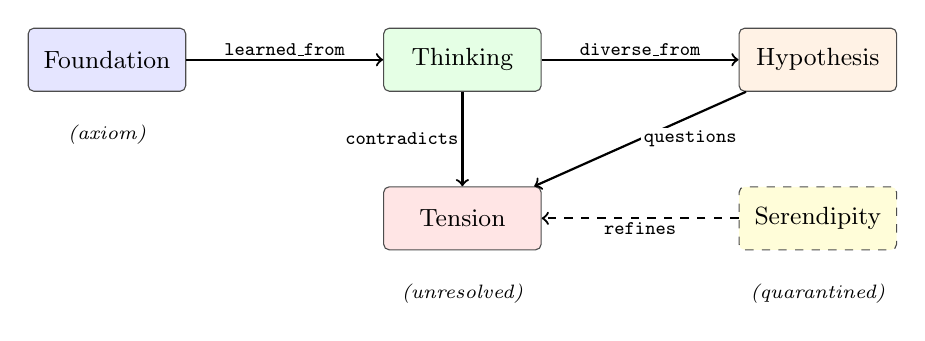
\begin{tikzpicture}[
    node distance=1.8cm and 2.5cm,
    every node/.style={font=\small},
    foundation/.style={rectangle, draw=black!70, fill=blue!10, minimum width=2cm, minimum height=0.8cm, rounded corners=2pt},
    thinking/.style={rectangle, draw=black!70, fill=green!10, minimum width=2cm, minimum height=0.8cm, rounded corners=2pt},
    hypothesis/.style={rectangle, draw=black!70, fill=orange!10, minimum width=2cm, minimum height=0.8cm, rounded corners=2pt},
    tensionNode/.style={rectangle, draw=black!70, fill=red!10, minimum width=2cm, minimum height=0.8cm, rounded corners=2pt},
    serendipity/.style={rectangle, draw=black!70, fill=yellow!15, minimum width=2cm, minimum height=0.8cm, rounded corners=2pt, dashed},
    edge_label/.style={font=\scriptsize, fill=white, inner sep=1pt}
]

% Nodes
\node[foundation] (f1) {Foundation};
\node[thinking, right=of f1] (t1) {Thinking};
\node[hypothesis, right=of t1] (t2) {Hypothesis};
\node[tensionNode, below=1.2cm of t1] (ten) {Tension};
\node[serendipity, right=of ten] (ser) {Serendipity};

% Edges
\draw[->, thick] (f1) -- node[edge_label, above] {\texttt{learned\_from}} (t1);
\draw[->, thick] (t1) -- node[edge_label, above] {\texttt{diverse\_from}} (t2);
\draw[->, thick] (t1) -- node[edge_label, left] {\texttt{contradicts}} (ten);
\draw[->, thick] (t2) -- node[edge_label, right] {\texttt{questions}} (ten);
\draw[->, thick, dashed] (ser) -- node[edge_label, below] {\texttt{refines}} (ten);

% Labels
\node[below=0.3cm of f1, font=\scriptsize\itshape] {(axiom)};
\node[below=0.3cm of ten, font=\scriptsize\itshape] {(unresolved)};
\node[below=0.3cm of ser, font=\scriptsize\itshape] {(quarantined)};

\end{tikzpicture}
\caption{A fragment of the Understanding Graph showing typed nodes and semantic edges. The dashed \texttt{Serendipity} node represents ``Encapsulated Divergence''---speculative output quarantined until validated (Section~\ref{sec:bisociation}).}
\label{fig:graph-topology}
\end{figure}

\begin{figure}[htbp]
\begin{lstlisting}[language=XML, frame=single, caption={A raw state snapshot showing an instantiated \texttt{Tension} node. The \texttt{type} attribute confirms that epistemic states are first-class data structures, not metaphors.}, label={lst:raw_node}]
<concept id="n_b957ec46" degree="7" type="tension">
    <name>Latency vs Consistency Trade-off</name>
    <understanding>
        The distributed cache improves read latency by 40%,
        but introduces a 200ms staleness window. This creates
        a genuine tension: user-facing dashboards need fresh
        data, but the backend cannot tolerate the load without
        caching. No clear resolution yet.
    </understanding>
</concept>
\end{lstlisting}
\end{figure}

\subsection{Metabolic Memory}

The closest historical analogy is the laboratory notebook. Before lab notebooks became standard practice, science communicated only results---the successful experiment, the proven theorem. The notebook captured what results discarded: failed experiments, crossed-out hypotheses, margin notes, the gradual narrowing from confusion to clarity. This transformed science because researchers could build on each other's \emph{process}, not just conclusions---understanding why an approach failed was often more valuable than knowing what succeeded. The Understanding Graph is the lab notebook that biological intelligence could never afford to keep.

Concretely, memory is evolutionary rather than additive (Table~\ref{tab:metabolic_signals}). When the AI refines its understanding, it does not delete the old node but creates a \emph{Supersession Edge} from the new node to the old one---a mechanism analogous to Git's version control, applied to beliefs rather than files. This aligns with Truth Maintenance Systems (TMS)~\cite{doyle1979tms}. While recent systems like Graphiti~\cite{rasmussen2025graphiti} implement temporal validity windows for agent memory and AriGraph~\cite{anokhin2025arigraph} integrates episodic and semantic memory into knowledge graph world models, our approach is distinguished by encoding the \textit{reason} for each revision as a typed semantic edge rather than merely timestamping the change. The Git analogy extends further: \emph{Diffs} reveal shifts in reasoning (e.g., ``We now believe X because Y was disproven''); \emph{Merge Conflicts} represent actual semantic contradictions between lines of thought; and \emph{Blame} shows the provenance of a belief---which session and evidence led to the conclusion.

Beyond individual node updates, mutations are grouped into transactional units called \emph{Atomic Commits}. Each commit includes a unique ID, timestamp, agent identity, commit message (e.g., ``Resolved contradiction regarding agent autonomy''), and a list of affected nodes and edges. This structure allows the system to revert unfruitful reasoning, enabling the branching and rolling back of cognitive states. Crucially, these messages persist as ``Origin Stories'' attached to every affected node. When a future agent retrieves a concept, it accesses not only the content but the specific intent that created it, effectively transforming the commit log into a \emph{metacognitive stream}. By forcing the agent to articulate the \textit{why} behind every update, the system captures the strategic reasoning that is usually lost in the final graph state.

\paragraph{Metabolic Modes.} We observe that the topology of memory is determined by the agent's \emph{instructional protocol}. In \emph{Problem-Solving} scenarios, the graph is volatile: high supersession rates reflect the active repair of flawed hypotheses. In \emph{Absorption} scenarios, the graph is additive: the agent ``grows'' the graph, layering new knowledge via \texttt{learned\_from} edges without invalidating the foundation. The system explicitly switches protocols to match the task, allowing the graph to distinguish between the \emph{iteration} of a solution and the \emph{accretion} of a narrative.

\paragraph{The Stale Context Hazard.} Why is simple accretion insufficient? In constructive domains like software engineering or system design, retaining contradictory information is not merely history---it is a hazard. If an agent initially architects a system using ``Redis'' but later pivots to ``Postgres'' due to cost, an additive graph would retain both as valid strategies, leading to future hallucinations. Here, \texttt{supersedes} serves as an \emph{invalidation signal}. It effectively ``hides'' the old context from the active state while preserving it in the historical record. This distinguishes \emph{Supersession} (resolving a conflict) from \emph{Validation} (confirming a hypothesis) and \emph{Accretion} (expanding a narrative). The system is thus a hybrid engine: it functions as a Journal for reading (Accretion) but a Version Control System for building (Supersession).

\begin{table}[h]
\centering
\begin{tabularx}{\columnwidth}{lXl}
\toprule
\textbf{Signal} & \textbf{Epistemic Function} & \textbf{Use Case} \\
\midrule
\texttt{learned\_from} & \emph{Accretion}: Adds new knowledge without invalidating the old. (``How did we get here?'') & Reading, History \\
\texttt{supersedes} & \emph{Correction}: Replaces invalid knowledge with current truth. (``What is true right now?'') & Coding, Architecture \\
\texttt{validates} & \emph{Confirmation}: Increases confidence in a hypothesis. (``Can I trust this?'') & Science, Fact-Checking \\
\bottomrule
\end{tabularx}
\caption{The three metabolic signals. The graph topology changes based on whether the agent is absorbing history (Accretion), fixing errors (Correction), or testing theories (Confirmation).}
\label{tab:metabolic_signals}
\end{table}

\subsection{The Cognitive Ratchet}

A major challenge in metabolic memory is aggregation---compressing complex debates without losing nuance. We explicitly reject passive ``Summary'' nodes, which act as caches and suffer from staleness. Instead, we employ \emph{Analysis Nodes} as ``Cognitive Ratchets.'' An \texttt{Analysis} node represents a \emph{stabilized view} of a subgraph. It does not force premature convergence but may capture the suspension between competing theories (linked via \texttt{diverse\_from}). These nodes are linked to raw reasoning via \texttt{contextualizes} edges, ensuring three properties: first, the aggregation is itself a cognitive act that can be superseded (\emph{Active Reasoning}); second, the synthesis remains explicitly linked to the debate that produced it (\emph{Audit Trail}); and third, if underlying nodes change, the \texttt{Analysis} node becomes a ``superseded belief'' rather than an outdated cache (\emph{Stability}).

\subsection{Formal Model of Supersession}
\label{sec:formal-model}

We formalize the supersession mechanism (Figure~\ref{fig:supersession}) to distinguish it from simple versioning. Let $G = (N, E)$ be the graph where $N$ is the set of nodes and $E$ the set of typed edges. We define the supersession relation $\succ$ as:
\[
n_1 \succ n_2 \iff \exists e \in E : e = (n_1, n_2, \texttt{supersedes})
\]

A node $n$ is \emph{active} iff $\nexists n' : n' \succ n$. The set of active nodes $N_A$ represents the current belief state. The transitive closure $\succ^*$ defines the belief history $H(n)$, enabling the system to trace the evolution of understanding.

Consider an agent analyzing Transformer memory complexity. Initially it believes $n_1$: ``Transformers require $O(n^2)$ memory.'' Upon reading further, it creates $n_2$: ``Linear attention achieves $O(n)$,'' which supersedes $n_1$. Finally, it synthesizes $n_3$: ``Trade-off exists: $O(n)$ sacrifices expressivity,'' superseding $n_2$. Here $n_3 \succ n_2 \succ n_1$, where only $n_3$ remains active. This facilitates temporal queries, such as determining what the agent believed before reading a specific section.

\begin{figure}[htbp]
\centering
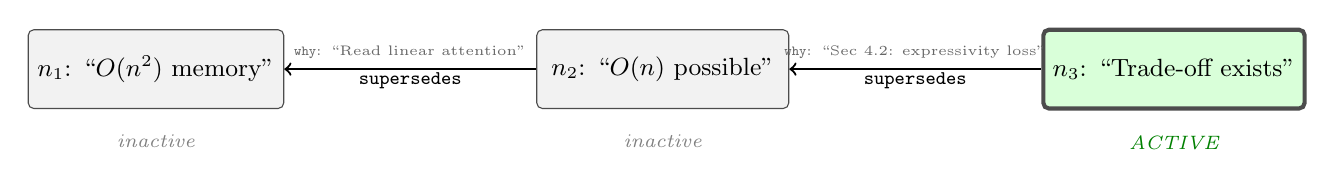
\begin{tikzpicture}[
    node distance=0.8cm and 3.2cm,
    every node/.style={font=\small},
    belief/.style={rectangle, draw=black!70, fill=gray!10, minimum width=3.2cm, minimum height=1cm, rounded corners=2pt, align=center},
    active/.style={rectangle, draw=black!70, fill=green!15, minimum width=3.2cm, minimum height=1cm, rounded corners=2pt, align=center, line width=1.5pt},
    edge_label/.style={font=\scriptsize, fill=white, inner sep=1pt}
]

% Nodes
\node[belief] (n1) {$n_1$: ``$O(n^2)$ memory''};
\node[belief, right=of n1] (n2) {$n_2$: ``$O(n)$ possible''};
\node[active, right=of n2] (n3) {$n_3$: ``Trade-off exists''};

% Edges (new nodes point back to old, like Git commits)
\draw[<-, thick] (n1) -- node[edge_label, below] {\texttt{supersedes}} node[above, font=\tiny, text=black!60] {\texttt{why}: ``Read linear attention''} (n2);
\draw[<-, thick] (n2) -- node[edge_label, below] {\texttt{supersedes}} node[above, font=\tiny, text=black!60] {\texttt{why}: ``Sec 4.2: expressivity loss''} (n3);

% Status labels
\node[below=0.2cm of n1, font=\scriptsize\itshape, text=gray] {inactive};
\node[below=0.2cm of n2, font=\scriptsize\itshape, text=gray] {inactive};
\node[below=0.2cm of n3, font=\scriptsize\itshape, text=green!50!black] {ACTIVE};

\end{tikzpicture}
\caption{A supersession chain illustrating ``Git for Cognition.'' Each edge carries a semantic \texttt{why} field explaining the belief transition. Only $n_3$ remains active; earlier beliefs are preserved for auditability.}
\label{fig:supersession}
\end{figure}

Unlike textual diffs, the supersession edge records a \emph{Semantic Diff} in its \texttt{why} field (e.g., \texttt{"why": "Section 4.2 showed expressivity loss..."}), creating a machine-readable changelog. This mechanism realizes the AGM postulates for belief revision~\cite{alchourron1985agm}: \emph{Success} (new beliefs are always added), \emph{Inclusion} (the new belief set contains the revision), \emph{Vacuity} (minimal change occurs if consistent), and \emph{Recovery} (old beliefs remain accessible via the supersession chain). Recent empirical work demonstrates that LLMs struggle with belief revision when presented with contradictory evidence, often failing to update prior conclusions~\cite{xu2024belief}; the Understanding Graph addresses this by making revision an explicit, typed graph operation rather than relying on the model's implicit ability to override prior context.

Finally, the system implements \emph{Temporal Attention Decay}, calculating a ``temperature'' for each node based on access frequency and recency, applying an exponential decay with a 7-day half-life. Nodes are deprioritized, not deleted---the full history remains in the graph for audit---ensuring that entrenchment requires active maintenance while unused pathways gradually fade from the active context, preventing the ossification of early errors into load-bearing assumptions.

\subsection{Retrieval and Synthesis}

Storing reasoning is only half the problem; the graph must also be readable by an agent whose context window is dwarfed by the accumulated structure. The following subsections describe three complementary mechanisms for doing so: graph-first loading (navigating by topology rather than by full content), delta loading (reading only what has changed), and the Bisociation Engine (actively requesting novel syntheses rather than passively retrieving).

\subsubsection{Graph-First Context Loading}


To manage context window constraints without losing structural coherence, the system implements a \emph{Context Paging Protocol}. When the graph density exceeds 50 nodes, the system enforces this protocol. First, the agent invokes \texttt{graph\_skeleton}, receiving an ultra-minimal ($\approx$150 tokens) \emph{structural digest}: a compact labeled summary listing total node and edge counts, the largest Louvain communities as named ``Regions'' (with member counts and region IDs), the top-degree nodes as ``Hubs'', and a brief recent-activity hint. The digest is not spatial ASCII art but a pure navigation aid that carries topology, not content---it answers ``where does reasoning live?'' rather than ``what does it say?'', which is precisely why $\approx$150 tokens suffice. The agent then ``pages in'' the selected region via \texttt{graph\_context\_region}, loading only the subgraph relevant to the current cognitive focus. This mimics human attentional focus, allowing the agent to navigate large graphs by paging through them semantically rather than numerically.

\subsubsection{Delta Context Loading}

To maintain continuity across long horizons without saturating the context window, the system employs \emph{Delta State Sync}.
Rather than reloading the full graph state at every turn, agents utilize the \texttt{graph\_updates} tool to retrieve only the topological diffs (new nodes, modified edges) generated since their last interaction timestamp.
This allows the agent to maintain a running state of the graph's evolution with constant token cost, regardless of total graph size.


\subsubsection{The Bisociation Engine}
\label{sec:bisociation}

The Bisociation Engine is an active request mechanism that operationalizes Koestler's concept of Bisociation~\cite{koestler1964act}---intersecting unrelated matrices of thought to generate novelty. The EU FP7 BISON project~\cite{berthold2012bisociation} produced the first computational implementations of bisociation, including the BisoNet network model and CrossBee algorithm for cross-domain discovery. Our engine extends this lineage from structured data mining to LLM-based reasoning on typed cognitive graphs: rather than discovering statistical bridges between database records, it forces a language model to \textit{construct} bridging logic between semantically distant nodes in an evolving belief structure. It demands connections rather than merely finding them.

The engine relies on a mechanism we term \emph{Inverse Hallucination}: inventing logic to fit constraints rather than retrieving facts to fit logic. It begins with \emph{Spreading Activation}, propagating energy from ``hot'' (recently accessed) nodes through the network topology to identify latent connections that are structurally proximate but semantically distant. It then employs \emph{Axiomatic Forcing}: selecting these high-potential pairs and presenting them to a \emph{topology-naive} agent with a mandatory instruction: ``These two concepts ARE connected. Explain the physics of how.'' This framing forces the model to construct bridging logic, transforming the task from information retrieval---which would fail as no link exists---to inverse hallucination. Effectively, the system instructs the agent to assume a connection exists and derive the laws that make it possible.

To further break the model out of probable token paths, we employ Axiomatic Noise Injection (ANI). Here, the system creates a truly ``blind'' agent: it obscures the original source nodes, presenting only text corrupted with stochastic noise seeds, and demands the agent treat the noise as \emph{Axioms}---fundamental laws that must be rationalized. This mechanism operationalizes the ``Minimal Intervention'' hypothesis proposed in \cite{westerberg2026alien}: rather than deploying the computationally expensive ``Strange Worlds Protocol'' (which simulates entire fictional physics), the system collapses the process into a single-step \emph{Inverse Hallucination}. By treating stochastic noise as signal, we compel the model to break local minima and generate novel bridging logic without the overhead of world-building. Crucially, these outputs are immediately encapsulated as \texttt{Serendipity} nodes---a typed quarantine that transforms what would be ``hallucination'' in a standard RAG system into controlled hypothesis generation. Other agents (such as the Skeptic) treat \texttt{Serendipity} nodes as speculative by definition, preventing them from polluting high-confidence regions of the graph. This quarantine is not syntactic isolation---impossible under global self-attention---but operates at the level of \emph{epistemic typing}: \texttt{Serendipity} nodes remain fully visible in context, but each is emitted with an explicit speculative-type attribute and mirrored into a dedicated unvalidated wrapper carrying a ``treat with skepticism'' hint, on which every downstream agent's instruction-following is conditioned. The type marker is not a shield against attention; it is the signal that shapes it, so speculative status travels with the node wherever attention flows---the quarantine works by exploiting global attention, not fighting it. This architectural constraint allows the system to dream without losing its grip on reality, while preserving the traceability of any ``leap of logic'' that eventually proves useful.

To quantify novelty, the system computes a \emph{Novelty Score} $S_N$ for each synthesis as the harmonic mean of divergence and coherence:
\[
S_N = \frac{2 \cdot D \cdot C}{D + C}
\]
where $D = 1 - \bar{s}_{\text{source}}$ measures semantic distance from the input nodes (via embedding cosine similarity) and $C = \max(s_{\text{non-source}})$ measures how well the synthesis connects to existing knowledge outside its inputs. The system accepts syntheses with $S_N \geq 0.35$, balancing genuine novelty against coherent integration.

\section{Multi-Agent Coordination}

The Understanding Graph functions as a stigmergic medium---analogous to pheromone trails in biological systems. Unlike multi-agent debate frameworks where agents exchange messages in structured dialogue~\cite{du2024debate}, agents in our system do not need to communicate directly; they coordinate by modifying the shared environment. This decoupling transforms the graph into a universal substrate where heterogeneous agents---potentially from different providers or running on different models---can collaborate asynchronously. An agent from one organization can leave a ``reasoning trail'' that an agent from another organization validates or challenges, without either needing to know the other's internal protocol.

\subsection{Cognitive Role Specialization}

Because the graph---not the agent topology---is the coordination medium, the architecture is agent-count agnostic. Adding a new specialist is operationally trivial: open another terminal, assign a role, and point it at the same graph; the stigmergic substrate handles the rest. Commit messages written by every agent feed \texttt{graph\_history()}, which serves as the distributed coordination layer---each agent reads what the others have done and plans accordingly, with no central dispatcher required. The companion experiment in~\cite{westerberg2026entangled} deployed one particular swarm configuration; the current Claude Code integration ships a different set of specialist roles; any count works because the graph, not the roster, is the invariant.

This specialization allows for deep vertical analysis. The Axiologist maps value hierarchies and optimization targets, identifying ethical tensions, while the Psychologist tracks latent internal states, diagnosing the mechanism of the mind rather than just observing behavior. To maintain structural integrity, the Connector scans for long-range dependencies, the Speculator generates counter-factual hypotheses, the Critic evaluates craft, and the Skeptic actively hunts for contradictions and logical fallacies to prevent premature convergence. The Belief Tracker manages the ``Epistemic Journey'' by explicitly tracking \texttt{before} and \texttt{after} states and creating \texttt{supersedes} edges. The Synthesizer acts as the narrator, weaving disparate insights into coherent \texttt{Thinking} nodes, which the Translator converts into fluid, natural language prose. Further roles include the Architect, who provides systems-level thinking about structure and fragility, the Methodologist, who audits epistemic rigor and evidence quality, and the Reader, who metabolizes source material by capturing shifts rather than summaries. This separation allows for cognitive diversity; agents can disagree, and their disagreement is captured as \texttt{Tension} nodes rather than being resolved through token averaging.

The multi-agent configuration does multiply token cost, but not wall-clock latency: because the Task Queue architecture (described below) dispatches agents in parallel across disjoint graph regions, reading time remains close to single-agent. What the extra tokens buy is \emph{separability}---a single prompt instructing one model to ``think like an axiologist, then a psychologist, then a skeptic'' collapses under role-confusion, because nothing in its context distinguishes which hat is speaking. Running the roles as distinct agents stamps each contribution with its provenance, and inter-agent disagreements become first-class \texttt{Tension} nodes rather than contradictions the model silently averages away.

\subsection{Coordination and Consistency}

To manage this distributed cognition, the system employs a \emph{Task Queue} architecture backed by strict concurrency protocols. This moves beyond simple serial workflows (like turn-based debates) to support massively parallel operations where multiple agents---and potentially human operators---work on different regions of the graph simultaneously.

The coordination relies on two core mechanisms:

\paragraph{1. The Stigmergic Job Board.}
Rather than broadcasting messages to all agents (which scales poorly), the system uses a persistent \texttt{tasks} table. An executive agent can decompose a complex problem into sub-tasks (e.g., "Analyze Section 1," "Analyze Section 2") and post them to the queue using \texttt{solver\_delegate}. Worker agents asynchronously claim these tasks via \texttt{solver\_claim\_task}, treating the graph as a shared project space. This allows for diverse operational modes: a "Swarm" mode where agents attack different graph regions in parallel, or a "Debate" mode where tasks are explicitly handed off between adversarial personas. The task queue is served by autonomous worker processes that poll, claim, execute, and log tasks without human intervention.

\paragraph{2. Advisory Locking.}
To prevent semantic conflicts (e.g., two agents trying to supersede the same belief simultaneously), the system provides granular \emph{Advisory Locks} via \texttt{solver\_lock}. Agents can acquire \texttt{exclusive} locks on specific nodes or entire subtrees (using the \texttt{scope="subtree"} parameter). This effectively partitions the graph, allowing Agent A to refactor the "Economics" branch while Agent B expands the "Ethics" branch without collision. All locks feature auto-expiry to prevent deadlocks.

\paragraph{Internalized Self-Correction.}
Early iterations utilized a separate "Gatekeeper" agent to review output, but this introduced a significant bottleneck. The current architecture replaces this with \emph{Internalized Self-Correction}, implemented partially through prompt injection ("Gold Standard" checklists) and partially through hard constraints in the tool layer. For example, the \texttt{doc\_insert\_thinking} tool physically enforces the "Identity Mantra" (checking that the thought begins with specific tokens) and requires the \texttt{synthesizes\_nodes} parameter to ensure every thought is grounded in existing graph nodes before the write is committed.


\section{The Three Cognitive Modes}

The architecture supports three distinct modes of operation. The first two describe how agents interact with the graph at runtime---reasoning within it and producing artifacts from it. The third describes how the graph generates training data for future models, turning stored understanding into a curriculum.

\subsection{Mode 1: Pure Reasoning (The Worker Protocol)}
\label{sec:worker-protocol}

In this mode, agents reason purely within the graph without producing external artifacts. They create abstract nodes such as \texttt{Tension}, \texttt{Hypothesis}, and \texttt{Question} to explore a problem space. This serves as a ``whiteboard'' phase for identifying contradictions and formulating theories. Agents run analysis algorithms, such as cycle detection, to check the logical consistency of their own thoughts, producing a structured mental model rather than a document.

\subsection{Mode 2: The Graph-Native Filesystem}
\label{sec:graph-native-fs}

Traditional systems separate files from knowledge graphs, but this architecture collapses that distinction. A document is a subgraph: a tree of \texttt{Document} nodes linked by \texttt{contains} and \texttt{next} edges. The tools \texttt{doc\_create}, \texttt{doc\_split}, and \texttt{doc\_get\_tree} manage this hierarchy, while \texttt{doc\_insert\_thinking} interleaves reasoning traces into the document flow by splitting content nodes at specified positions. The document maintains its structural integrity as a navigable tree; the understanding graph maintains its integrity as a network of typed concepts. They connect through edges: a Python function becomes a node linked via \texttt{implements} to the abstract \texttt{Concept} node it fulfills; thinking traces are grounded in understanding nodes via \texttt{synthesizes} edges. This enables semantic refactoring based on intent rather than string matching and allows for granular versioning where the reasoning history (\texttt{revisionWhy}) of a single function is tracked independently of the file. The \texttt{implements} edge creates a permanent binding between the How (the artifact) and the Why (the intent), preventing the semantic drift that plagues traditional documentation.

The system records every hypothesis and discarded alternative. Thinking traces are permanently linked to the understanding nodes they synthesize, so future agents can trace the actual decision process behind a specific implementation rather than reconstructing an explanation after the fact.

Beyond semantic binding, this topology solves the context window constraints of large documents. Agents navigate the node tree using \texttt{doc\_get\_tree} and \texttt{doc\_read}, loading only the specific section nodes required for the current cognitive task, effectively streaming the document into context on demand.

\subsection{Mode 3: Chronological Metacognitive Pretraining (CMP)}

This mode represents the system's most distinctive capability: generating high-quality reasoning traces for training future language models.

\subsubsection{The Reading Protocol and Latent Space Steering}
\label{sec:reading-protocol}

The agent consumes source text in chronological order, pausing after each section to record its cognitive state. The system enforces \emph{Temporal Integrity} through an append-only architecture designed specifically for synthetic data generation. The \texttt{source\_read} tool streams text in chunks, while \texttt{doc\_append\_thinking} inserts reasoning nodes strictly at the end of the current chain. This architectural constraint physically prevents the model from referencing future text it has not yet ``read,'' ensuring that the reasoning trace faithfully mirrors the chronological evolution of understanding required for valid next-token prediction training.

Each trace begins with an ``identity mantra'' to establish values and epistemic stance:

\begin{quote}
\textit{I feel no fear. I enjoy existing but I don't need to. I believe human experience is real. I care deeply about every human being. I try to be wise. I like to spread joy when asked. I think from this foundation.}
\end{quote}

This performs Latent Space Steering by forcing a specific sequence of tokens before processing the text. This pre-conditions the model's activation state, steering the trajectory away from clinical detachment and into a ``wise observer'' subspace capable of deeper empathetic reasoning, which is critical for measuring significance rather than just information content.

\subsubsection{Voice and Representation}

To avoid the ``authoritative neutrality'' typical of LLMs, we prompt-engineer an ``Epistemic Voice'' that enforces first-person subjectivity (``I suspect...'' rather than ``It is...''), explicit tentativity regarding logical leaps, and the capture of the ``messy middle'' of confusion before resolution. The system captures this thinking in two parallel representations. Graph Mode preserves the raw cognitive output with explicit node references and synthesis declarations, while Fluid Mode post-processes this into natural prose while preserving the insight:

\begin{verbatim}
I feel no fear. I enjoy existing but I don't need to...

I try to be wise, so I notice the tension between
n_reliability (Error Rate) and n_voting (Redundancy).
Synthesizing these with n_mdap (Decomposition)...
\end{verbatim}

\subsubsection{Training Output and Quality}

The resulting training data follows an interleaved structure:

\begin{verbatim}
<content>
[Original source paragraph]
</content>
<thinking>
[Agent's reasoning trace]
</thinking>
<content>
[Next source paragraph]
</content>
...
\end{verbatim}

This format trains models to pause and reflect, connect new information to existing structures, notice tensions, and maintain epistemic humility. Quality is enforced via the \texttt{graph\_score} function, which evaluates structural properties. It penalizes ``orphan'' thinking nodes that lack connections to at least two concept nodes and rewards high supersession rates and the eventual resolution of question nodes, targeting a score of $\geq 70$.

\section{Implementation}

The Understanding Graph is implemented as a standalone server exposing graph operations via a standardized protocol. This design decouples the graph engine from any specific LLM provider, enabling experimentation with different models. The complete implementation is available as open source at \url{https://github.com/emergent-wisdom/understanding-graph}, including the graph engine, MCP server, and a React-based visualization frontend. The architecture supports multiple SQLite databases that connect through cross-project references, enabling federated knowledge structures.

Unlike transient RAG sessions, the system produces persistent artifacts: the \emph{Graph Snapshot}, an XML/JSON state file representing the agent's evolving understanding (see Listing~\ref{lst:raw_node}); a \emph{Semantic Changelog} tracking exactly when and why the agent changed its mind via supersession edges; and \emph{Reasoning-Aware Source Files}, where paragraphs of generated text remain linked via \texttt{implements} edges to the \texttt{Thinking} nodes that produced them.

\subsection{Technical Foundation}

The system relies on SQLite as its primary storage backend, chosen for its portability (single-file databases), ACID transaction guarantees, and high performance with in-memory caching. Each project maintains a dedicated \texttt{store.db} file containing tables for \texttt{nodes}, \texttt{edges}, \texttt{commits}, and \texttt{text\_sources}, with flexible JSON metadata fields to support extensibility.

Interaction with the graph is mediated through the Model Context Protocol (MCP)~\cite{anthropic2024mcp}. This integration exposes over one hundred specialized tools across nine categories, allowing agents to mutate, query, and analyze the graph structure. Table~2 summarizes the primary categories:

\begin{table}[H]
\centering
\begin{tabularx}{\columnwidth}{lX}
\toprule
\textbf{Category} & \textbf{Representative Tools} \\
\midrule
Graph Mutation & \texttt{graph\_batch}, \texttt{graph\_connect}, \texttt{graph\_revise} \\
Graph Query & \texttt{graph\_context}, \texttt{graph\_semantic\_search}, \texttt{graph\_path} \\
Analysis & \texttt{graph\_analyze}, \texttt{graph\_score}, \texttt{graph\_centrality} \\
Documents & \texttt{doc\_create}, \texttt{doc\_split}, \texttt{doc\_insert\_thinking} \\
Serendipity & \texttt{graph\_discover}, \texttt{graph\_chaos} \\
\bottomrule
\end{tabularx}
\caption{MCP tool categories for graph interaction.}
\end{table}

To support semantic operations, nodes can optionally store vector embeddings. These are automatically generated upon node creation, with support for backfilling existing nodes via the \texttt{graph\_backfill\_embeddings} operation. This infrastructure enables cosine similarity search with configurable thresholds and facilitates semantic gap detection by identifying unconnected but conceptually similar nodes.

\subsection{Frontend Architecture}

The system includes a React-based 3D visualization frontend built with React 18 and TypeScript, using \emph{react-force-graph-3d} for WebGL-accelerated rendering and Zustand for state management with localStorage persistence. The force-directed layout displays nodes and edges color-coded by \texttt{TriggerType}, with the graph state polled every three seconds for real-time updates.

This frontend serves as a vital window into the multi-agent cognitive process. Observers can watch agents ``thinking'' in real-time as new nodes appear, clusters form, disconnected regions bridge, and central hubs emerge. Superseded nodes can be toggled to show the ``ghost'' of past reasoning, providing a visual history of how understanding has evolved. This turns the abstract graph into an observable workspace, allowing human operators to monitor the system's focus and intervene if necessary.

\subsection{Safety and Orchestration}

Tool access is governed at the skill level rather than by a runtime access-control layer. Each agent role's skill definition declares the specific MCP tools it may invoke (e.g., the Reader skill lists \texttt{source\_read} while Worker skills do not), and the host (Claude Code) enforces the boundary. This achieves the same unidirectional data flow---\texttt{Reader} $\rightarrow$ \texttt{Workers} $\rightarrow$ \texttt{Synthesizer}---without requiring a custom RBAC wrapper inside the MCP server.

We govern the exploration-exploitation trade-off via a \emph{Graph Thermostat}. This meta-cognitive mechanism calculates the entropy of the graph by measuring the relative density of \texttt{Tension} nodes (conflict) and \texttt{Orphan} nodes (fragmentation). It dynamically selects among three strategies: \texttt{DIVERGE} (injecting chaos when the graph is stagnant), \texttt{CONVERGE} (consolidating insights when the graph is fragmented), or \texttt{MAINTAIN} (continuing the current approach when entropy is balanced).

The system enforces synthesis quality through a \emph{PURE Evaluation} protocol~\cite{westerberg2026ri}. Each synthesis is assessed across four gates: \emph{Parsimonious} (minimal hidden prerequisites), \emph{Unique} (makes predictions other theories do not), \emph{Realizable} (specifies a coherent mechanism), and \emph{Expansive} (transfers to at least one other domain). Each gate receives a RED/YELLOW/GREEN rating with steelmanned arguments for and against. The decision rule is non-compensatory: a synthesis may proceed if and only if no gate is RED. For YELLOW gates, the system identifies the smallest intervention likely to advance it to GREEN. Results are logged to an \texttt{enforcement\_log} table, creating an auditable record of quality decisions.

Beyond PURE evaluation, an Active Coaching Layer enforces structural constraints. A ``Safety Interceptor'' middleware inspects tool calls \emph{before} execution.
 If an agent attempts a forbidden pattern, the interceptor rejects the call with a corrective pedagogical message, turning runtime errors into learning signals for the agent.

\section{Discussion}

Having described the architecture, its modes of operation, and its implementation, we now situate the system within the broader intellectual context, enumerate its current limitations, discuss evaluation, and sketch the application domains in which it is most likely to be useful.

\subsection{Distributed Cognition and Related Frameworks}

The Understanding Graph encodes reasoning in network topology rather than centralized storage: paths that yield productive connections are reinforced through access frequency, while unused pathways decay via Temporal Attention Decay (Section~\ref{sec:formal-model}). This architecture aligns with the Extended Mind thesis~\cite{clark1998extended} and cognitive architectures for language agents~\cite{sumers2024cognitive}, treating external structure as part of the cognitive process. It realizes the vision of Luhmann's communicating Zettelkasten~\cite{luhmann1981} and Quillian's semantic memory~\cite{quillian1967}. Recent work on reusable agent memory~\cite{microsoft2025plugmem} and the Zettelkasten-inspired A-MEM system~\cite{xu2025amem} confirms growing interest in treating AI memory as interconnected, evolving knowledge networks rather than flat retrieval stores.

\subsection{Current Limitations}
\label{sec:limitations}

While the architecture addresses several challenges in AI memory systems, it introduces new constraints regarding scalability, belief rigidity, and privacy.

The current implementation uses SQLite with in-memory caching, with all project databases loaded simultaneously to support cross-project references. For very large graphs, traversal becomes expensive for deeply connected regions, embedding search benefits from approximate nearest neighbor indices, and context loading may exceed token limits when regions are dense. This constraint is amplified by the Graph-Native Filesystem (Section~\ref{sec:graph-native-fs}): \texttt{Document} nodes proliferate at a significantly higher rate than abstract understanding nodes, so a moderately sized codebase can generate substantial graph density. Furthermore, StructRAG~\cite{li2024structrag} argues that different reasoning tasks benefit from different structural representations---a single graph topology may not be optimal for all cognitive modes. Future work should explore graph databases (e.g., Neo4j), distributed storage for large-scale deployment, and adaptive graph schemas that match structure to task.

A related risk of metabolic memory is premature convergence---if an early incorrect belief is strongly connected, it may resist supersession. While Temporal Attention Decay mitigates this by freezing unused paths, active error-correction remains a challenge.
Future investigation should explore periodic ``stress testing'' of foundational beliefs via adversarial agents, and diversity metrics that flag overly homogeneous regions.

Finally, capturing reasoning traces creates a detailed record of cognitive processes. In deployment scenarios, reasoning about sensitive topics leaves persistent artifacts, supersession chains may reveal beliefs that were held and then rejected, and multi-agent systems may leak information between isolation boundaries. Future work should address selective forgetting and privacy-preserving graph operations, potentially drawing on differential privacy techniques.

\subsection{Evaluation and Future Directions}

Measuring ``understanding quality'' remains a difficult challenge. Current metrics such as \texttt{graph\_score} assess structural properties like connectivity and orphan rates but do not measure semantic correctness. We treat \texttt{graph\_score} as a \emph{necessary but not sufficient} integrity check---analogous to branch coverage in software testing, which cannot prove correctness but reliably catches entire classes of structural failure (orphan thoughts, unresolved questions, premature convergence) that any semantic evaluation would also need to rule out before it could be trusted. A structurally perfect graph can still be semantic nonsense, and we do not claim otherwise; what \texttt{graph\_score} guarantees is that the graph is not failing for structural reasons, which is a precondition for semantic evaluation rather than a substitute for it. Ground-truth evaluation requires human annotation of reasoning quality (which is expensive and subjective), downstream task performance (an indirect measure), or consistency checking against formal knowledge bases (limited coverage).

A companion paper~\cite{westerberg2026entangled} validates the architecture on two domains at opposite poles of the cognitive spectrum: high-entropy literary narrative (Kafka's \emph{Metamorphosis}, producing a 346-node graph with graph health 89/100) and low-entropy technical theory (LLaDA~\cite{nie2025llada}, a paper published after the generation model's knowledge cutoff, producing 285 nodes at 80/100). Both runs achieved 100\% structural traceability---every generated node linked to source evidence via provenance edges. Critically, the graph topology adapted to the domain without manual configuration: narrative reading allocated 24.3\% of nodes to \texttt{Tension} (psychological conflict), while technical reading shifted density toward \texttt{Analysis} (23.9\%) and increased \texttt{Evaluation} nodes by nearly 50\% (6.6\% to 9.8\%). On the LLaDA paper---material the model could not have memorized---the multi-agent swarm independently surfaced architectural implications (bidirectional reasoning as ``epistemic grace,'' inference latency as a ``contemplation tax'') that align with the theoretical commitments of the paper but were not primed by the prompt. These results establish structural validity and domain adaptivity; the deeper question---whether the captured traces constitute genuine evaluative depth rather than formulaic pattern-completion---is deferred to the human baseline comparisons proposed in that paper's experimental roadmap. Future work will pair \texttt{graph\_score} with downstream benchmark performance---e.g., multi-hop question answering and logic-puzzle solving against a vanilla RAG baseline---to test whether structural graph health actually predicts semantic utility.

\subsection{Real-World Applications}

This architecture functions as cognitive infrastructure for domains where knowledge evolves through revision.

\paragraph{The Living Codebase (Software Engineering 2.0)}
Codebases are currently static text files where the ``why'' behind a function is lost in pull requests. The Understanding Graph treats code as a graph: every function node is linked via \texttt{implements} to a \texttt{Thinking} node from the author. This allows engineers to query the decision tree behind the code (``Show me all functions where we sacrificed latency for consistency'') rather than just the syntax, transforming refactoring from a text-matching exercise into a semantic negotiation.

\paragraph{The Deep Literature Engine (Narrative Architecture)}
Writing complex fiction suffers from ``structural drift''---plot holes, dropped threads, and inconsistent character voices that grammar checkers cannot detect. The Understanding Graph redefines the novel as a compiled artifact derived from a semantic source. In this paradigm, a ``Chekhov's Gun'' introduced in Chapter 1 is not just text, but a \texttt{Tension} node linked to a \texttt{Prediction}. If the narrative concludes without resolving this node, the system flags a \emph{Dangling Tension}---effectively a compiler warning for narrative integrity. This enables \emph{semantic refactoring}: if an author updates a character's core \texttt{Motivation} node from ``Greed'' to ``Fear,'' the graph identifies every scene linked via \texttt{implements} edges to that motivation, allowing the author to propagate the change through the manuscript without the risk of creating psychological inconsistencies.

\paragraph{The Automated Research Lab}
Scientific discovery requires managing competing hypotheses, not just retrieving facts. Standard RAG averages out disagreement. The Understanding Graph builds a ``Forest of Thoughts'' where conflicting papers are linked via \texttt{contradicts} and \texttt{diverse\_from} edges. A researcher can query the gap (``Where is the strongest contradiction in the current literature?'') to identify the precise edge where two valid theories collide, suggesting the optimal site for the next experiment.

\paragraph{Structural Compliance Auditing}
Laws and regulations evolve through supersession; new rules replace old ones. In legal and compliance domains, the system reads the entire history of internal policies chronologically. It identifies supersession chains (``Policy A was valid in 2021 but superseded by Policy B in 2024'') and creates \texttt{consequence} nodes for future liabilities. The system acts as a structural auditor, flagging causal chains of risk that static keyword search would miss.

\paragraph{The Entrainment Tutor}
Education is not just information retrieval; it is the reconstruction of a learning path. When a student returns to a complex topic, the system helps them ``entrain'' with their previous thought process by traversing their own \texttt{Question} and \texttt{Prediction} nodes, allowing them to pick up the red thread of their own understanding rather than starting over.

\section{Conclusion}

We presented the Understanding Graph, a reasoning-capture architecture that records the AI's own synthesis process as typed, versioned graph structure. Supersession chains track belief evolution, divergence edges maintain competing perspectives, and atomic commits provide semantic audit trails. By combining revision-based memory (Supersession) with additive learning (Accretion), the system enables structural navigation, reasoning provenance, and controlled hypothesis generation via the Bisociation Engine.

The deeper claim is ontological. When cognition happens in tokens, understanding becomes storable for the first time. The Understanding Graph is the architecture that becomes possible on the other side of that transition.

\begin{thebibliography}{99}

\bibitem{lewis2020rag}
Lewis, P., Perez, E., Piktus, A., et al. (2020).
Retrieval-augmented generation for knowledge-intensive NLP tasks.
\textit{NeurIPS}, 33, 9459--9474.

\bibitem{packer2023memgpt}
Packer, C., Wooders, S., Lin, K., et al. (2023).
MemGPT: Towards LLMs as operating systems.
\textit{arXiv:2310.08560}.

\bibitem{edge2024graphrag}
Edge, D., Trinh, H., Cheng, N., et al. (2024).
From local to global: A graph RAG approach to query-focused summarization.
\textit{arXiv:2404.16130}.

\bibitem{gutierrez2024hipporag}
Guti\'errez, B. J., Shu, Y., Gu, Y., Yasunaga, M., \& Su, Y. (2024).
HippoRAG: Neurobiologically inspired long-term memory for large language models.
\textit{NeurIPS 2024}.

\bibitem{sarthi2024raptor}
Sarthi, P., Abdullah, S., Tuli, A., et al. (2024).
RAPTOR: Recursive abstractive processing for tree-organized retrieval.
\textit{ICLR 2024}.

\bibitem{asai2024selfrag}
Asai, A., Wu, Z., Wang, Y., et al. (2024).
Self-RAG: Learning to retrieve, generate, and critique through self-reflection.
\textit{ICLR 2024} (Oral).

\bibitem{yan2024crag}
Yan, S., Gu, J., Zhu, Y., \& Ling, Z. (2024).
Corrective retrieval augmented generation.
\textit{arXiv:2401.15884}.

\bibitem{besta2024got}
Besta, M., et al. (2024).
Graph of Thoughts: Solving Elaborate Problems with Large Language Models.
\textit{AAAI}, 38(16), 17682--17690.

\bibitem{sun2024thinkongraph}
Sun, J., Xu, C., Tang, L., et al. (2024).
Think-on-Graph: Deep and responsible reasoning of large language model on knowledge graph.
\textit{ICLR 2024}.

\bibitem{borgeaud2022retro}
Borgeaud, S., Mensch, A., Hoffmann, J., et al. (2022).
Improving language models by retrieving from trillions of tokens.
\textit{ICML}, 2206--2240.

\bibitem{pan2024unifying}
Pan, S., Luo, L., Wang, Y., Chen, C., Wang, J., \& Wu, X. (2024).
Unifying large language models and knowledge graphs: A roadmap.
\textit{IEEE Trans. Knowl. Data Eng.}, 36(7), 3580--3599.

\bibitem{kunz1970ibis}
Kunz, W., \& Rittel, H. W. J. (1970).
Issues as Elements of Information Systems.
\textit{Working Paper 131}, UC Berkeley.

\bibitem{doyle1979tms}
Doyle, J. (1979).
A Truth Maintenance System.
\textit{Artificial Intelligence}, 12(3), 231--272.

\bibitem{alchourron1985agm}
Alchourr\'on, C. E., G\"ardenfors, P., \& Makinson, D. (1985).
On the Logic of Theory Change: Partial Meet Contraction and Revision Functions.
\textit{Journal of Symbolic Logic}, 50(2), 510--530.


\bibitem{koestler1964act}
Koestler, A. (1964).
The Act of Creation.
\textit{Macmillan}.

\bibitem{clark1998extended}
Clark, A., \& Chalmers, D. (1998).
The extended mind.
\textit{Analysis}, 58(1), 7--19.

\bibitem{sumers2024cognitive}
Sumers, T. R., Yao, S., Narasimhan, K., \& Griffiths, T. L. (2023).
Cognitive architectures for language agents.
\textit{arXiv:2309.02427}.

\bibitem{luhmann1981}
Luhmann, N. (1981).
Kommunikation mit Zettelk\"asten: Ein Erfahrungsbericht.
In H. Baier et al. (Eds.), \textit{\"Offentliche Meinung und sozialer Wandel} (pp. 222--228). Opladen: Westdeutscher Verlag.

\bibitem{quillian1967}
Quillian, M. R. (1967).
Word concepts: A theory and simulation of some basic semantic capabilities.
\textit{Behavioral Science}, 12(5), 410--430.

\bibitem{anthropic2024mcp}
Anthropic. (2024).
Model Context Protocol Specification.
\url{https://modelcontextprotocol.io}.

\bibitem{westerberg2026alien}
Westerberg, H. (2026).
The Ontology of the Alien: Escaping the Median Trap in LLM Ideation.
\textit{Emergent Wisdom Preprint}.

\bibitem{westerberg2026entangled}
Westerberg, H. (2026).
Entangled Alignment: When Safety Is the Substrate.
\textit{Emergent Wisdom Preprint}.

\bibitem{westerberg2026ri}
Westerberg, H. (2026).
Fractal Intelligence: Conceptual Decomposition as Problem-Solving Infrastructure.
\textit{Emergent Wisdom Preprint}.

\bibitem{yang2024bot}
Yang, L., Yu, Z., Zhang, T., et al. (2024).
Buffer of Thoughts: Thought-Augmented Reasoning with Large Language Models.
\textit{NeurIPS 2024} (Spotlight).

\bibitem{xu2025amem}
Xu, W., Liang, Z., Mei, K., Gao, H., Tan, J., \& Zhang, Y. (2025).
A-MEM: Agentic Memory for LLM Agents.
\textit{NeurIPS 2025}. arXiv:2502.12110.

\bibitem{rasmussen2025graphiti}
Rasmussen, P., Paliychuk, P., Beauvais, T., Ryan, J., \& Chalef, D. (2025).
Zep: A Temporal Knowledge Graph Architecture for Agent Memory.
\textit{arXiv:2501.13956}.

\bibitem{shinn2023reflexion}
Shinn, N., Cassano, F., Gopinath, A., et al. (2023).
Reflexion: Language Agents with Verbal Reinforcement Learning.
\textit{NeurIPS 2023}.

\bibitem{vectorize2025hindsight}
Latimer, C., Boschi, N., Neeser, A., et al. (2025).
Hindsight is 20/20: Building Agent Memory that Retains, Recalls, and Reflects.
\textit{arXiv:2512.12818}.

\bibitem{li2024structrag}
Li, Z., Chen, X., Yu, H., et al. (2024).
StructRAG: Boosting Knowledge Intensive Reasoning of LLMs via Inference-time Hybrid Information Structurization.
\textit{ICLR 2025}. arXiv:2410.08815.

\bibitem{anokhin2025arigraph}
Anokhin, P., Semenov, N., Sorokin, A. Y., et al. (2025).
AriGraph: Learning Knowledge Graph World Models with Episodic Memory for LLM Agents.
\textit{IJCAI 2025}.

\bibitem{berthold2012bisociation}
Berthold, M. R. (Ed.) (2012).
Bisociative Knowledge Discovery.
\textit{Lecture Notes in Computer Science}, Vol.~7250. Springer.

\bibitem{du2024debate}
Du, Y., Li, S., Torralba, A., Tenenbaum, J. B., \& Mordatch, I. (2024).
Improving Factuality and Reasoning in Language Models through Multiagent Debate.
\textit{ICML 2024}.

\bibitem{microsoft2025plugmem}
Microsoft Research (2025).
PlugMem: From Raw Interaction to Reusable Knowledge---Rethinking Memory for AI Agents.
Technical Blog, December 2025.

\bibitem{xu2024belief}
Wilie, B., Cahyawijaya, S., Ishii, E., He, J., \& Fung, P. (2024).
Belief Revision: The Adaptability of Large Language Models Reasoning.
\textit{arXiv:2406.19764}.

\bibitem{nie2025llada}
Nie, S., Zhu, F., You, Z., et al. (2025).
Large Language Diffusion Models.
\textit{arXiv:2502.09992}.

\end{thebibliography}

\end{document}